%!Tex Root = ../main.tex
% ./Packete.tex
% ./Design.tex
% ./Deklarationen.tex
% ./Aufgabe1.tex
% ./Aufgabe2.tex
% ./Aufgabe3.tex
% ./Aufgabe4.tex
% ./Bonus.tex

\section{Organisatorisches}

\begin{frame}{Organisatorisches}{Studienleistung }
  \begin{itemize}
    \item Anmeldung zur \alert{Übung} in unserem \alert{Übungsportal}
    \item Anmeldung zur \alert{Studienleistung} im \alert{HisInOne}
    \item Zu erbringende Leistungen:
    \begin{itemize}
      \item Mindestens \alert{75\%} der Aufgaben in den Übungsblättern müssen sinnvoll bearbeitet werden.
      \begin{itemize}
        \item Das Bearbeiten \alert{einer Teilaufgabe} einer Aufgabe zählt bereits als sinnvolles Bearbeiten der gesamten Aufgabe.
        \item Die Aufgabe muss \alert{nicht korrekt} gelöst sein, es muss nur sichtbar sein, dass \alert{versucht} wurde diese Aufgabe zu lösen.
      \end{itemize}
      \item Eine Aufgabe aus den Übungen muss im Tutorat \alert{vorgerechnet} werden.
      \item \alert{Regelmäßige, aktive Teilnahme} an den Übungsgruppen \Smiley[1.5][PrimaryColorDimmed].
    \end{itemize}
  \end{itemize}
\end{frame}

\begin{frame}{Organisatorisches}{Infos zum Tutorat}
  \begin{itemize}
    \item \alert{Tutorat wird aufgezeichnet:} \url{https://www.youtube.com/playlist?list=PLmsC317bB1b0T198lvGTddbqThQ6gDDG2}
    \item \alert{\LARGE \uppercase{Bitte}} gebt RETI-Code \alert{getippt} ab und nicht handschrifftlich.
    \begin{figure}
      \centering
      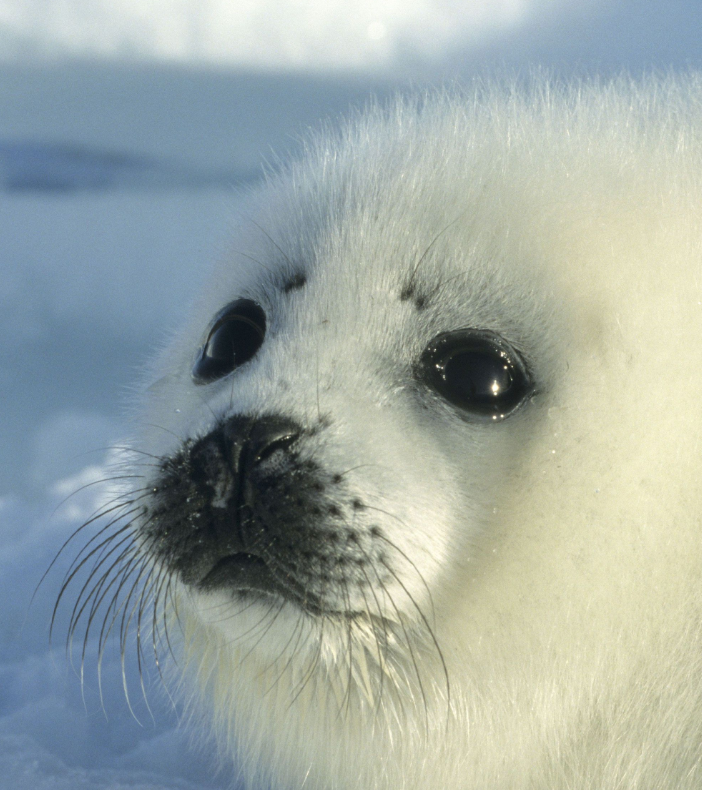
\includegraphics[height=0.3\paperheight]{./figures/babyrobe.png}
    \end{figure}
    \item \alert{Kritik} am Tutorat: \url{https://forms.gle/gLJHVMZhQWcSK2N18}
  \end{itemize}
\end{frame}

\begin{frame}{Organisatorisches}{Hilfsmittel}
  \begin{itemize}
    \item \alert{Mindmap zum Vorlesungsstoff:} \url{https://github.com/matthejue/Mindmaps/releases/download/main/Technische_Informatik.pdf}
    \item \alert{zum Überprüfen der RETI-Abgaben:} \url{https://github.com/matthejue/PicoC-Compiler/releases}
    \begin{itemize}
      \item \alert{Dokumentation:} \url{https://github.com/matthejue/Bachelorarbeit_Dokumentation_out/blob/main/Dokumentation.pdf}
      \item \alert{Einführung:} \url{https://github.com/matthejue/PicoC-Compiler/blob/master/doc/getting_started.md}
      \item \alert{Bugs melden:} \url{https://github.com/matthejue/PicoC-Compiler/issues}
    \end{itemize}
  \end{itemize}
\end{frame}

\begin{frame}{Organisatorisches}{Gruppenbildung}
  \begin{itemize}
    \item Wer würde sich gerne mit einer \alert{anderen Person} aus dem Tutorat (Tutor ausgenommen) zu einer \alert{Gruppe zusammenschließen}?
    \item Die \alert{Studenten} freuen sich wegen \alert{Arbeitsteilung} über \alert{weniger Tipparbeit}. Der \alert{Tutor} freut sich auch über \alert{weniger Korrekturen}.
  \end{itemize}
  
\includegraphics[width=0.2\textwidth, center]{./figures/vereinbarung.png}
\end{frame}
